\section{Przypadek Testowy 4 - Tabu Search - Wpływ liczby rozpatrywanych sąsiadów na otrzymane wyniki}
  \subsection{Cel:}
  Celem tego testu jest sprawdzenie w jaki sposób liczba rozpatrywanych sąsiadów w każdej
  iteracji algorytmu wpływa na wynik. \\
  W tym teście sąsiedzi wyznaczani są przy pomocy ruchów typu \textit{invert}. Do wykonania tego testu wykorzystano wygenerowane grafy typu \textit{FULL MATRIX} o liczbie miast ze zbioru 
  $ n \in \{100,150,...,600\} $. Dla każdego testu wykonano 1000 iteracji z maksymalną stagnacją równą 20 iteracji bez poprawy. 
  Dodatkowo rozmiar listy tabu jest stały równy 15 elementów.
  Sprawdzane rozmiary rozpatrywanych sąsiadów należą do zbioru $k \in \{100\%,50\%,25\%,10\%,$\}. \\
  Rozmiar podawany jest w procentach względem rozmiaru danej instancji $(100\%=n, 50\%=\frac{n}{2},...)$
  
  \subsection{Wyniki: }
    Otrzymane wyniki przedstawia poniższa tabela: \\
    \textbf{Uwaga:} Ze względow objętościowych w sprawozdaniu zostały zawarte jedyne informacje na temat pojedynczego testu
    \begin{table}[H]
      \centering
      \begin{tabular}{||c c c c||} 
       \hline
       n & cost & time & Nsize \\ [0.5ex] 
       \hline\hline
        100 &	2005	& 1,35	& $10\%$ \\
        100	& 1575	& 2,39	& $25\%$ \\
        100	& 1267	& 4,08	& $50\%$ \\
        100 &	1068	& 7,53	& $100\%$ \\
        150 &	2601	& 2,29	& $10\%$ \\ 
        150 &	2053	& 4,35	& $25\%$ \\
        150 &	1807	& 8,22	& $50\%$ \\
        150 &	1438	& 15,84	& $100\%$ \\
        200 &	3393	& 3,75	& $10\%$ \\
        200 &	2538	& 7,8	& $25\%$ \\
        200 &	2188	& 14,07	& $50\%$ \\
        200	& 1818	& 27,89	& $100\%$ \\
        250	& 3999	& 4,92	& $10\%$ \\
        250	& 2979	& 10,97	& $25\%$ \\
        250	& 2538	& 21,19	& $50\%$ \\
        250	& 2220	& 41,99	& $100\%$ \\
        300	& 4737	& 6,85	& $10\%$ \\
        300	& 3486	& 16,04	& $25\%$ \\
        300	& 3015	& 31,39	& $50\%$ \\
        300	& 2762	& 66,19	& $100\%$ \\
        350	& 5258	& 10,6	& $10\%$ \\
        350	& 4366	& 21,29	& $25\%$ \\
        350	& 3664	& 41,41	& $50\%$ \\
        350	& 2983	& 85,81	& $100\%$ \\
        400	& 5666	& 13,41	& $10\%$ \\
        400	& 4640	& 29,54	& $25\%$ \\
        400	& 4142	& 59,31	& $50\%$ \\
        400	& 3386	& 110,54	& $100\%$ \\
        450	& 6303	& 14,92	& $10\%$ \\
        450	& 5084	& 35,32	& $25\%$ \\
        450	& 4398	& 66,15	& $50\%$ \\
        450	& 3652	& 140,77	& $100\%$ \\
        500	& 7060	& 18,77	& $10\%$ \\
        500	& 5616	& 43,4	& $25\%$ \\
        500	& 4799	& 85,06	& $50\%$ \\
        500	& 4192	& 170,88	& $100\%$ \\
        550	& 7559	& 24	& $10\%$ \\
        550	& 6318	& 55,35	& $25\%$ \\
        550	& 5240	& 101,99	& $50\%$ \\
        550	& 4262	& 207,54	& $100\%$ \\
        600	& 8330	& 26,54	& $10\%$ \\
        600	& 6520	& 52,15	& $25\%$ \\
        600	& 5441	& 126,8	& $50\%$ \\
        600	& 4677	& 252,83	& $100\%$ \\
       \hline
      \end{tabular}
      \caption{Tabela przedstawiająca otrzymane wyniki, Nsize- rozmiar sąsiedztwa, czas podawany w sekundach}
      \end{table}
  \subsection{Wykresy: }
    \begin{figure}[H]
      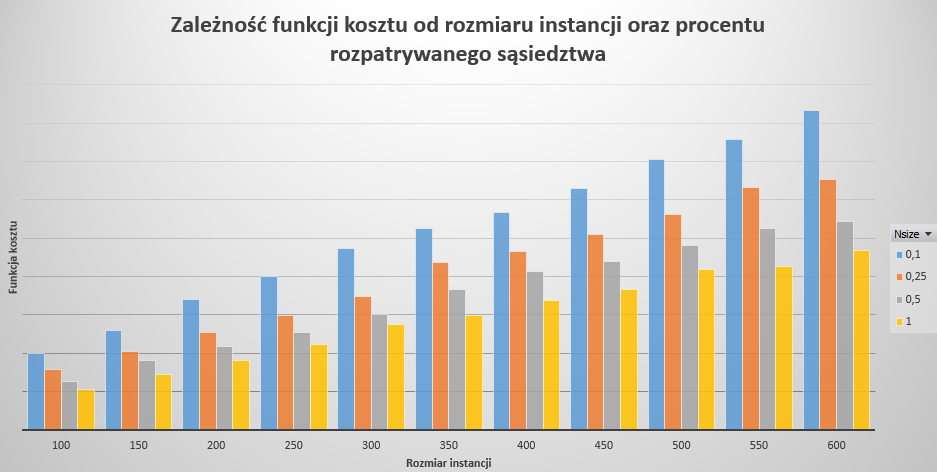
\includegraphics[scale=0.5]{test4photo1.png}
      \centering
      \caption{zależność funkcji kosztu od rozmiaru instancji oraz procentu rozpatrywanego sąsiedztwa}
    \end{figure}
    \begin{figure}[H]
      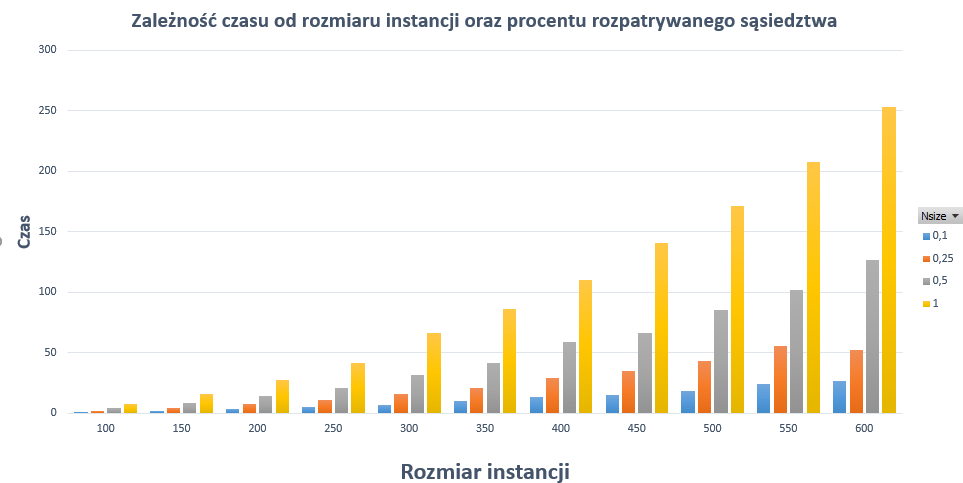
\includegraphics[scale=0.5]{test4photo2.png}
      \centering
      \caption{zależność czasu od rozmiaru instancji oraz procentu rozpatrywanego sąsiedztwa}
    \end{figure}
  \subsection{Wnioski: }
  Zauważamy, iż zwiększenie liczby potencjalnych kandydatów w każdej iteracji znacząco wpływa na otrzymane wyniki testowanego algorytmu, jak i na czas,
  w jakim ów algorytm wykonuje swoją pracę. Testy pokazały, iż optymalnym ustawieniem jest $50\%$, w którym otrzymujemy satysfakcjonujące rozwiązanie w rozsądnym czasie.\\
  Warto zauważyć, iż na otrzymane wyniki czasowe mają wpływ takie czynniki jak język programowania, w którym algorytm został zaimplementowany oraz zużycie procesora
  komputera, na którym wykonywano powyższe testy.

